\documentclass[../ClassicThesis.tex]{subfiles}
\begin{document}

%************************************************
\chapter{Assembly}\label{ch:assembly}
%************************************************

Assembling the laser cut plates to form the desired object is not trivial. Since multiple plates may be very similar to each other, it is not always clear which have to be put together. Thus, we decided to add assembly instructions, which allow the user to assemble the model hassle-free. Section~\sectionref{sub:assemblyplates} describes how these instructions are added to plates which were found either inherently or by extruding. The assembly instructions for stacked plates are discussed in Section~\sectionref{sub:assemblystacked}.

\section{Added Numbers Help Arranging Plates}

This section describes the currently used methods for adding assembly instructions. While these simplify assembly, they are not optimal. Ideas for improvement are discussed in Section~\sectionref{sec:assemblyimprovements}.

\subsection{Plates Connected With Finger Joins Are Annotated on Each Edge}\label{sub:assemblyplates}

Plates created by the \emph{PlateMethod} are connected by finger joints. In order to show which plates have to be put together, the corresponding edges are annotated accordingly.

\begin{figure}
    \centering
    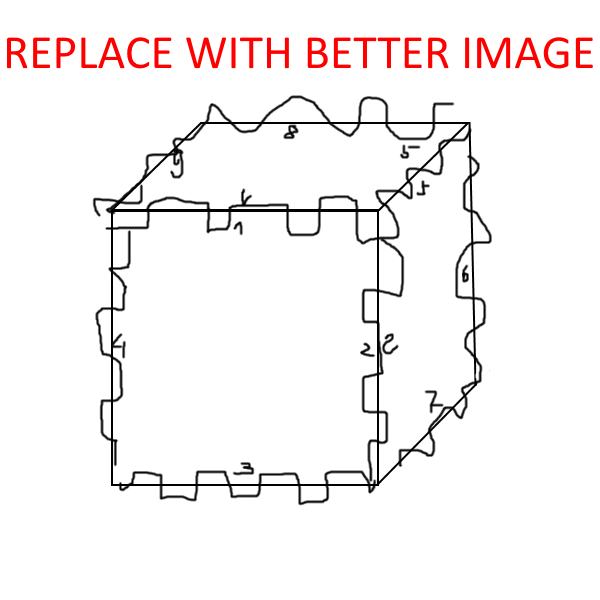
\includegraphics[width=0.5\columnwidth]{Images/assembly_plates.png}
    \caption{Assembly instructions for plates connected by finger joints.}
    \label{fig:assemblyplates}
\end{figure}

These annotations are created for each edge separately, by calling the \emph{addInstruction} function for each. This function is shown in Listing~\ref{lst:addinstructions}. The connection data is passed by setting this property beforehand. Thus, the nodes (which contain the plates) and the connection parameters can be extracted. Using these, the instructions are built for both plates.

\begin{listing}
\begin{minted}[
linenos
]{coffeescript}
addInstructions: ->
  { node1, node2, parameters } = @connection
  @buildInstruction(node1, parameters.node1Direction)
  @buildInstruction(node2, parameters.node2Direction)
\end{minted}
\caption{Adding instructions to connections.}
\label{lst:addinstructions}
\end{listing}

Listing~\ref{lst:buildinstruction} shows how this is done. First, we ensure that the data for the direction and the intersection line is valid. The intersection line tells us where to place the annotation, with the direction being the direction from the intersection line towards plate. This helps to place the annotation on the plate instead of placing it directly on the edge (with half of it not actually being located on the plate). The index of the connection is the number we want to annotate the edge with. Thus, we build a text box containing this number. Afterwards, the box is moved onto the intersection line. Using the direction, we can place it on the plate. Lastly, the created text box is added to the node.

\begin{listing}
\begin{minted}[
linenos,breaklines
]{coffeescript}
buildInstruction: (node, direction) ->
  if direction is null then return
  { index, intersectionLine } = @connection.parameters
  if not intersectionLine? then return 
  box = @buildInstructionBox(index)
  @moveObjXYToLineXY(box, @layLineIntoXY(intersectionLine[0], node.shape))
  box.translateOnAxis(direction, 0.75 * jointSpecs.height)
  node.assemblyInstruction.add(box)
\end{minted}
\caption{Building the assembly instruction for one plate.}
\label{lst:buildinstruction}
\end{listing}

\subsection{Stacked Plates Are Enumerated}\label{sub:assemblystacked}

The annotations added to stacked plates differ from the ones discussed above. Since the shafts already simplify the assembly of the model, we just enumerate the layers of plates. Sorting the plates by the number written on them tells the user how to assemble them. Figure~\ref{fig:assemblystacked} shows a side view of how the plates are annotated. While iterating over all layers and all plates contained in these layers, we add an annotation to each plate.

\begin{figure}
    \centering
    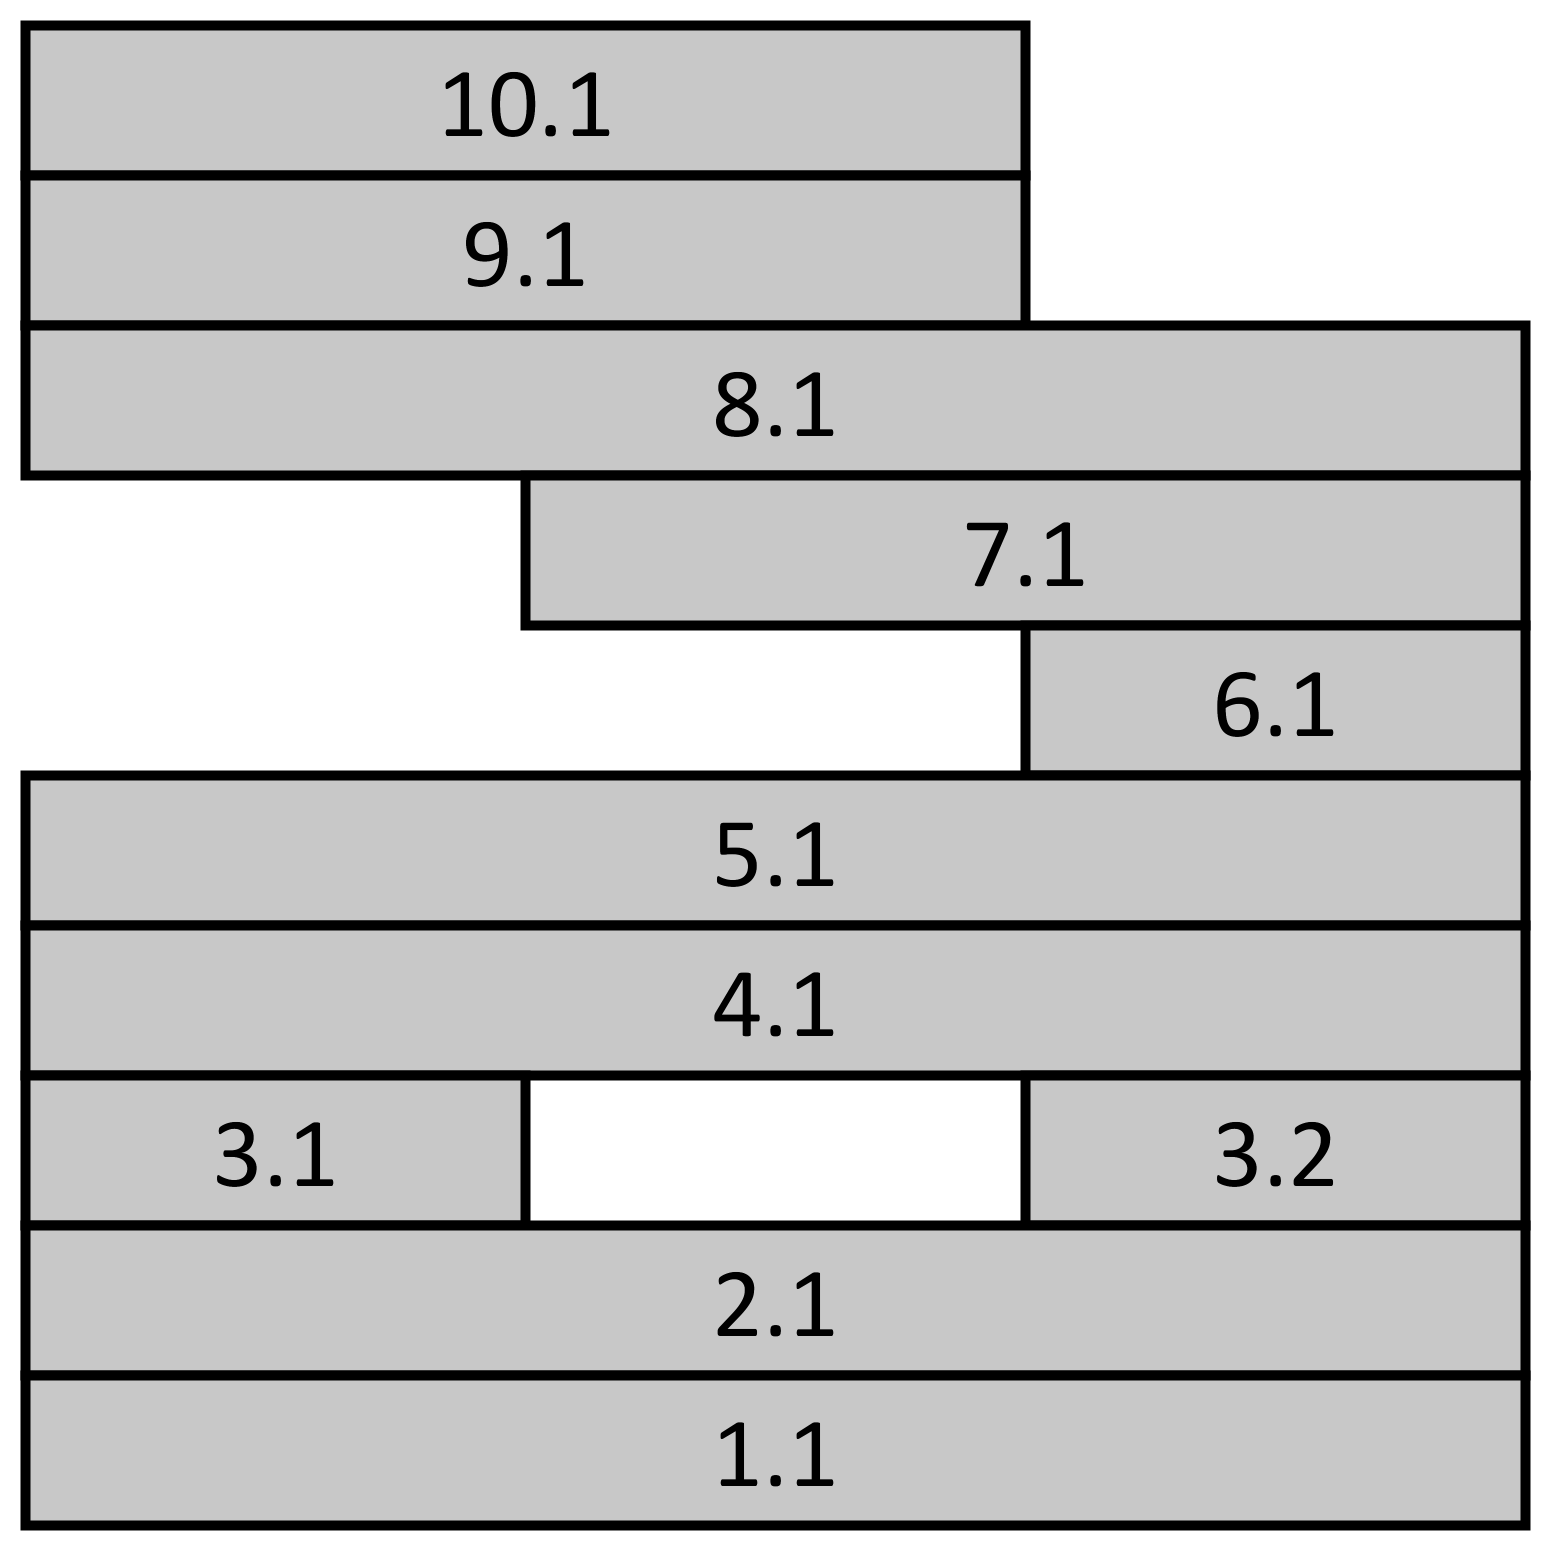
\includegraphics[width=0.5\columnwidth]{Images/assembly_stacked.png}
    \caption{Side view of assembly intructions for stacked plates. In reality, the annotations are placed on the main side of the plate.}
    \label{fig:assemblystacked}
\end{figure}

\section{Possible Improvements}\label{sec:assemblyimprovements}
\subsection{Icons Can Show the Orientation of Plates}

In addition to the annotations described in Section~\sectionref{sub:assemblyplates}, we propose adding icons which tell the user where the plate is located. Thus, the distinction between horizontal and vertical plates is made easy. The proposed icons are shown in Figure~\ref{fig:assemblyicons}. In addition to the arrow, which signalizes the arrangement of vertical plates, two icons describing horizontal plates are shown. These are based on the mathematical symbols indicating if an vector is pointing into or out of a diagram. All three symbols tell the user where - from the plates perspective - the top side of the model is located.

\begin{figure}
  \centering
  \begin{subfigure}[b]{0.3\textwidth}
    \centering
    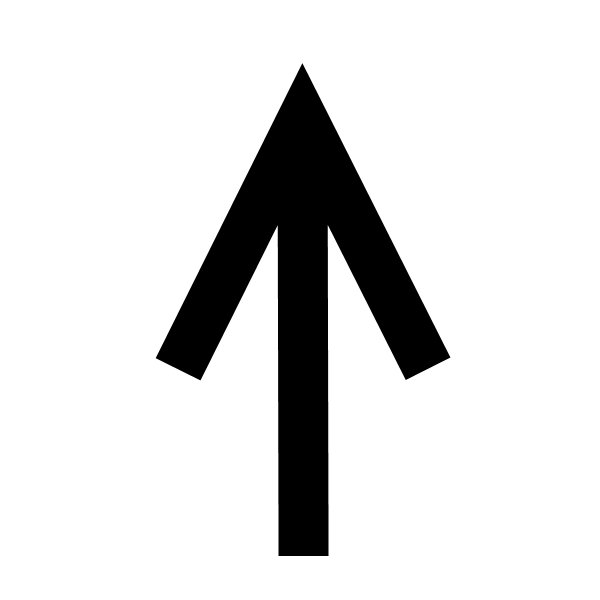
\includegraphics[width=\textwidth]{assembly_direction_side.png}
    \caption{Vertical plate. The arrow points to the top.}
    \label{fig:assemblyicons:side}
  \end{subfigure}
  \begin{subfigure}[b]{0.3\textwidth}
    \centering
    
\includegraphics[width=\textwidth]{assembly_direction_top.png}
    \caption{Horizontal plate, located at the top of the model.}
    \label{fig:assemblyicons:top}
  \end{subfigure}
  \begin{subfigure}[b]{0.3\textwidth}
    \centering
    
\includegraphics[width=\textwidth]{assembly_direction_bottom.png}
    \caption{Horizontal plate, located at the bottom of the model.}
    \label{fig:assemblyicons:bottom}
  \end{subfigure}
  \caption{Icons signalizing the orientation of a plate.}
  \label{fig:assemblyicons}
\end{figure}

\subsection{Annotating Plates Only Once Reduces Cutting Time}

Engraving the annotations onto plates usually takes longer than the actual cutting process. In Order to reduce this time, we propose to not annotate each edge individually. Instead, each plate should be engraved with a number, which clearly identifies it. Coupled with assembly instructions shown on screen, this still enables fast assembly, while reducing cutting time.

\end{document}